\chapter{KHẢO SÁT VÀ PHÂN TÍCH YÊU CẦU}

\section{Khảo sát hiện trạng}

\subsection*{Tổng quan}

Một tác nhân AI có thể tạo nhiều yêu cầu nối tiếp hoặc đồng thời trong quá trình hoàn thành một nhiệm vụ. Số lượng yêu cầu, mô hình được sử dụng và lượng tài nguyên tiêu thụ phụ thuộc vào kết quả trung gian, vì vậy tổng chi phí khó xác định trước.

Trong mô hình sử dụng trực tiếp, tổ chức hoặc lập trình viên thường cấp khóa của nhà cung cấp AI cho ứng dụng hoặc agent. Cách làm này đơn giản nhưng làm giảm khả năng kiểm soát tập trung: hệ thống khó biết agent nào tạo yêu cầu, tổ chức nào chịu chi phí, ngân sách còn lại bao nhiêu và yêu cầu có nằm trong chính sách được cấp hay không.

Vì vậy, đề tài định vị Asymptotic như một \textit{AI Agent Financial Gateway}. Tổ chức nạp tiền vào hệ thống, đăng ký các tác nhân AI bên ngoài và cấp khóa truy cập do Asymptotic quản lý. Khi agent cần gọi dịch vụ AI, request đi qua Gateway; Gateway kiểm tra định danh, ngân sách, hạn mức và chính sách trước khi gọi nhà cung cấp bằng thông tin xác thực nội bộ.

%-----------------------------------------------------------

\subsection*{Nhà cung cấp dịch vụ AI}

Nhà cung cấp dịch vụ AI tiếp nhận yêu cầu qua API và tính phí theo mô hình, số token hoặc loại dịch vụ. Chi phí thực tế thường chỉ được xác nhận khi phản hồi đã được tạo. Nhà cung cấp không quản lý ngân sách nội bộ của tổ chức sử dụng Gateway và cũng không biết yêu cầu thuộc tác nhân, nhiệm vụ hoặc hạn mức nào trong hệ thống Asymptotic.

Do đó, Gateway cần ước lượng chi phí trước khi gửi yêu cầu, sau đó ghi nhận mức sử dụng và chi phí sau khi nhận phản hồi. Với nguyên mẫu, hệ thống tập trung vào kiểm soát trước khi route request và lưu usage/cost/trace; quyết toán chính xác theo token thực tế ở mức production được xem là hướng mở rộng.

%-----------------------------------------------------------

\subsection*{Gateway tài chính cho AI Agent}

Gateway trong đề tài không chỉ là điểm vào kỹ thuật cho request. Hệ thống còn đóng vai trò kiểm soát tài chính theo thời gian thực cho các request do tác nhân AI phát sinh. Mỗi request cần được gắn với tổ chức, tác nhân, API key, chính sách sử dụng, ngân sách và nhà cung cấp AI tương ứng.

Điểm quan trọng là agent không dùng trực tiếp provider API key. Agent chỉ dùng khóa do Asymptotic cấp để gọi Gateway. Gateway mới là thành phần giữ và sử dụng thông tin xác thực nội bộ để gọi nhà cung cấp AI. Cách tổ chức này giúp hệ thống thu hồi quyền truy cập, áp chính sách và theo dõi chi phí mà không phải phát tán khóa của nhà cung cấp cho từng agent.

%-----------------------------------------------------------

\subsection*{Ngân sách, giao dịch và truy vết}

Việc chỉ tổng hợp chi phí sau khi dịch vụ đã được sử dụng không đủ cho bài toán của đề tài, vì khi đó hệ thống chỉ phát hiện vượt ngân sách sau khi chi phí đã phát sinh. Gateway cần tham gia trước khi request được gửi tới nhà cung cấp: kiểm tra ngân sách, giữ chỗ hoặc xác nhận hạn mức, sau đó mới cho phép request tiếp tục.

Ngoài kiểm soát trước thực thi, hệ thống cần lưu lại lịch sử request, usage, chi phí, trạng thái xử lý và quan hệ giữa tổ chức với tác nhân AI. Các dữ liệu này phục vụ báo cáo, kiểm tra và đối soát. Với các trường hợp request bị gửi lại do lỗi mạng hoặc mất phản hồi, cơ chế lũy đẳng giúp hạn chế ghi nhận trùng cho cùng một hành động.

%-----------------------------------------------------------

\subsection*{Mô hình thực thi của AI Agent}

Một nhiệm vụ của tác nhân AI có thể gồm các bước sinh nội dung, gọi công cụ, đánh giá kết quả và thử lại. Mỗi bước có thể tạo thêm yêu cầu mới. Do đó, hệ thống không thể giả định trước số lần gọi hoặc tổng chi phí của toàn bộ nhiệm vụ.

Trong phạm vi nguyên mẫu, mỗi yêu cầu được kiểm soát độc lập nhưng vẫn được liên kết với tổ chức, agent, API key và ngân sách tương ứng. Cách tiếp cận này phù hợp với MVP vì xử lý được rủi ro chi phí ở từng request mà không cần xây dựng môi trường chạy agent hoặc điều phối workflow của agent.

%-----------------------------------------------------------

\subsection*{Khoảng trống kỹ thuật và bài toán cần giải quyết}

Khoảng trống cần giải quyết gồm các điểm chính: thiếu định danh riêng cho AI Agent, thiếu kiểm soát ngân sách trước khi gọi dịch vụ, thiếu cơ chế quản lý provider credential tập trung, thiếu khả năng chống ghi nhận trùng và thiếu truy vết chi phí theo tổ chức/agent. Đề tài giải quyết các vấn đề này bằng một gateway có trạng thái, kết hợp đăng ký agent, API key, ví/ngân sách, chính sách sử dụng, danh mục provider/model, giao dịch PostgreSQL và lịch sử thực thi.

Phiên bản nguyên mẫu tập trung vào luồng cốt lõi của MVP: tổ chức nạp tiền, đăng ký agent, agent gọi Gateway bằng API key, Gateway kiểm tra ngân sách/chính sách, gọi AI Provider bằng credential nội bộ và ghi nhận usage/cost/trace. Các chức năng như hóa đơn, quyết toán production với provider và báo cáo quản trị hoàn chỉnh được xem là phạm vi mở rộng.

\section{Đặc tả yêu cầu hệ thống}

\subsection*{Phạm vi yêu cầu}

Các yêu cầu dưới đây mô tả hệ thống mục tiêu trong phạm vi MVP. Hệ thống tập trung vào kiểm soát tài chính theo từng request do AI Agent bên ngoài phát sinh. Hệ thống không tạo, huấn luyện, triển khai hoặc điều phối AI Agent; các agent được xem là phần mềm bên ngoài đã được tổ chức đăng ký vào Gateway.

Chương 4 đối chiếu từng yêu cầu với nguyên mẫu đã triển khai để phân biệt chức năng hoàn thành, chức năng hoàn thành một phần và chức năng chưa triển khai.

%-----------------------------------------------------------

\subsection*{Phân tích yêu cầu chức năng}

Hệ thống phải đáp ứng các yêu cầu chức năng sau:

\begin{description}
    \item[FR01 -- Quản lý tổ chức và ví/ngân sách] Hệ thống phải ghi nhận tổ chức sử dụng dịch vụ, số dư ví hoặc ngân sách khả dụng, đồng thời cập nhật các biến động tài chính phát sinh từ nạp tiền, phân bổ ngân sách và ghi nhận chi phí.
    \item[FR02 -- Đăng ký và quản lý tác nhân AI] Hệ thống phải cho phép tổ chức hoặc người được phân quyền đăng ký AI Agent bên ngoài vào Gateway, gắn Agent với tổ chức, trạng thái hoạt động, phạm vi ngân sách/chính sách và lịch sử sử dụng.
    \item[FR03 -- Cấp và xác thực API key cho tác nhân] Hệ thống phải cấp API key do Asymptotic quản lý cho từng Agent, lưu khóa ở dạng bảo vệ và xác thực khóa này trước khi xử lý request gửi vào Gateway.
    \item[FR04 -- Quản lý provider, model và biểu giá] Hệ thống phải lưu và quản lý thông tin AI Provider, model, endpoint, provider credential nội bộ, trạng thái hỗ trợ và biểu giá hoặc mức phí dự kiến phục vụ tính chi phí.
    \item[FR05 -- Thiết lập chính sách sử dụng] Hệ thống phải cho phép thiết lập hạn mức, quota, budget hoặc policy theo tổ chức, lập trình viên, Agent hoặc phạm vi sử dụng được cấp quyền.
    \item[FR06 -- Kiểm soát chi phí trước thực thi] Trước khi chuyển tiếp request tới AI Provider, hệ thống phải ước lượng chi phí dự kiến, kiểm tra ngân sách/chính sách liên quan và chỉ cho phép request tiếp tục khi các điều kiện này hợp lệ.
    \item[FR07 -- Định tuyến request tới AI Provider] Hệ thống phải chuyển tiếp request hợp lệ tới AI Provider bằng provider credential nội bộ của Asymptotic; Agent không được sử dụng trực tiếp provider API key.
    \item[FR08 -- Kiểm soát lũy đẳng] Hệ thống phải phát hiện request gửi lại dựa trên khóa lũy đẳng và nội dung request, trả kết quả đã lưu khi request trùng khớp và không tạo thêm giao dịch hoặc chi phí trùng.
    \item[FR09 -- Ghi nhận usage, cost và trace] Hệ thống phải lưu lịch sử request, trạng thái xử lý, Agent, tổ chức, provider, model, usage, cost, transaction và trace để phục vụ kiểm tra, báo cáo và đối soát.
    \item[FR10 -- Trả lỗi khi vượt giới hạn] Hệ thống phải trả lỗi rõ ràng và không gọi AI Provider khi request bị từ chối do sai khóa, Agent không hợp lệ, vượt quota, vượt budget hoặc vi phạm chính sách.
\end{description}

%-----------------------------------------------------------

\subsection*{Phân tích yêu cầu phi chức năng}

Các yêu cầu phi chức năng quy định các thuộc tính chất lượng của hệ thống:

\begin{description}
    \item[NFR01 -- Tính nhất quán tài chính] Trong mọi giao dịch nạp tiền, phân bổ ngân sách, tạm giữ và quyết toán chi phí, hệ thống phải không để số dư hoặc ngân sách khả dụng bị âm. Khi nhiều request đồng thời tiêu thụ cùng một ngân sách, tổng giá trị được chấp nhận không được vượt quá ngân sách khả dụng.
    \item[NFR02 -- Bảo mật khóa truy cập] API key của Agent, mật khẩu người dùng và provider credential không được lưu ở dạng rõ trong cơ sở dữ liệu hoặc log. Các chức năng quản trị khóa, provider credential và ngân sách phải được kiểm soát bằng phân quyền.
    \item[NFR03 -- Khả năng truy vết] Mỗi request đi qua Gateway phải truy vết được tổ chức, Agent, API key, provider, model, chính sách áp dụng, usage, cost, transaction, trạng thái xử lý và thời điểm phát sinh.
    \item[NFR04 -- Khả năng phục hồi] Khi xảy ra lỗi cơ sở dữ liệu, lỗi mạng hoặc lỗi AI Provider, hệ thống không được để lại trạng thái tài chính không thể đối soát. Giao dịch liên quan phải được hoàn trả, hoàn tất hoặc đánh dấu chờ đối soát.
    \item[NFR05 -- Hiệu năng] Thời gian xử lý của lớp Gateway cần được đo tách biệt với thời gian chờ AI Provider. Trong phạm vi nguyên mẫu, hệ thống phải ghi nhận đủ dữ liệu thời gian để đánh giá độ trễ do xác thực, kiểm tra chính sách, kiểm tra ngân sách và ghi trace tạo ra.
\end{description}

\section{Phân tích actor}

Các actor trong hệ thống được xác định theo vai trò tương tác với \textit{AI Agent Financial Gateway}. \cref{tab:actors} mô tả phạm vi trách nhiệm của từng actor trước khi trình bày biểu đồ trường hợp sử dụng.

\begin{longtable}{|L{4cm}|L{10cm}|}
\caption{Danh sách actor của hệ thống}
\label{tab:actors} \\\hline
\textbf{Actor} & \textbf{Mô tả vai trò} \\\hline
\endfirsthead
\hline
\textbf{Actor} & \textbf{Mô tả vai trò} \\\hline
\endhead
Người dùng & Người dùng bên ngoài bắt đầu quy trình đăng ký tổ chức và trở thành quản trị viên đầu tiên sau khi đăng ký thành công.\\\hline
Quản trị viên tổ chức & Vai trò quản trị trong phạm vi một tổ chức, thực hiện nạp tiền, phân bổ ngân sách, quản lý lập trình viên và theo dõi chi phí sử dụng.\\\hline
Lập trình viên & Thành viên thuộc tổ chức, đăng ký và quản lý tác nhân AI, thiết lập hạn mức, quản lý API key và theo dõi dữ liệu sử dụng trong phạm vi được cấp.\\\hline
AI Agent & Phần mềm tự động bên ngoài hệ thống, gọi Gateway bằng API key do Asymptotic cấp để sử dụng dịch vụ AI có kiểm soát.\\\hline
Nhà cung cấp dịch vụ AI & Hệ thống bên ngoài xử lý yêu cầu AI do Gateway chuyển tiếp bằng credential nội bộ của Asymptotic.\\\hline
Nhà cung cấp dịch vụ thanh toán & Hệ thống bên ngoài hỗ trợ xử lý giao dịch nạp tiền vào ví tổ chức.\\\hline
Quản trị viên hệ thống & Vai trò vận hành hệ thống, quản lý provider, model, biểu giá và chính sách định tuyến/fallback.\\\hline
\end{longtable}

\section{Phân tích trường hợp sử dụng}

\subsection*{Biểu đồ trường hợp sử dụng tổng quát}
\begin{figure}[H]
    \centering
    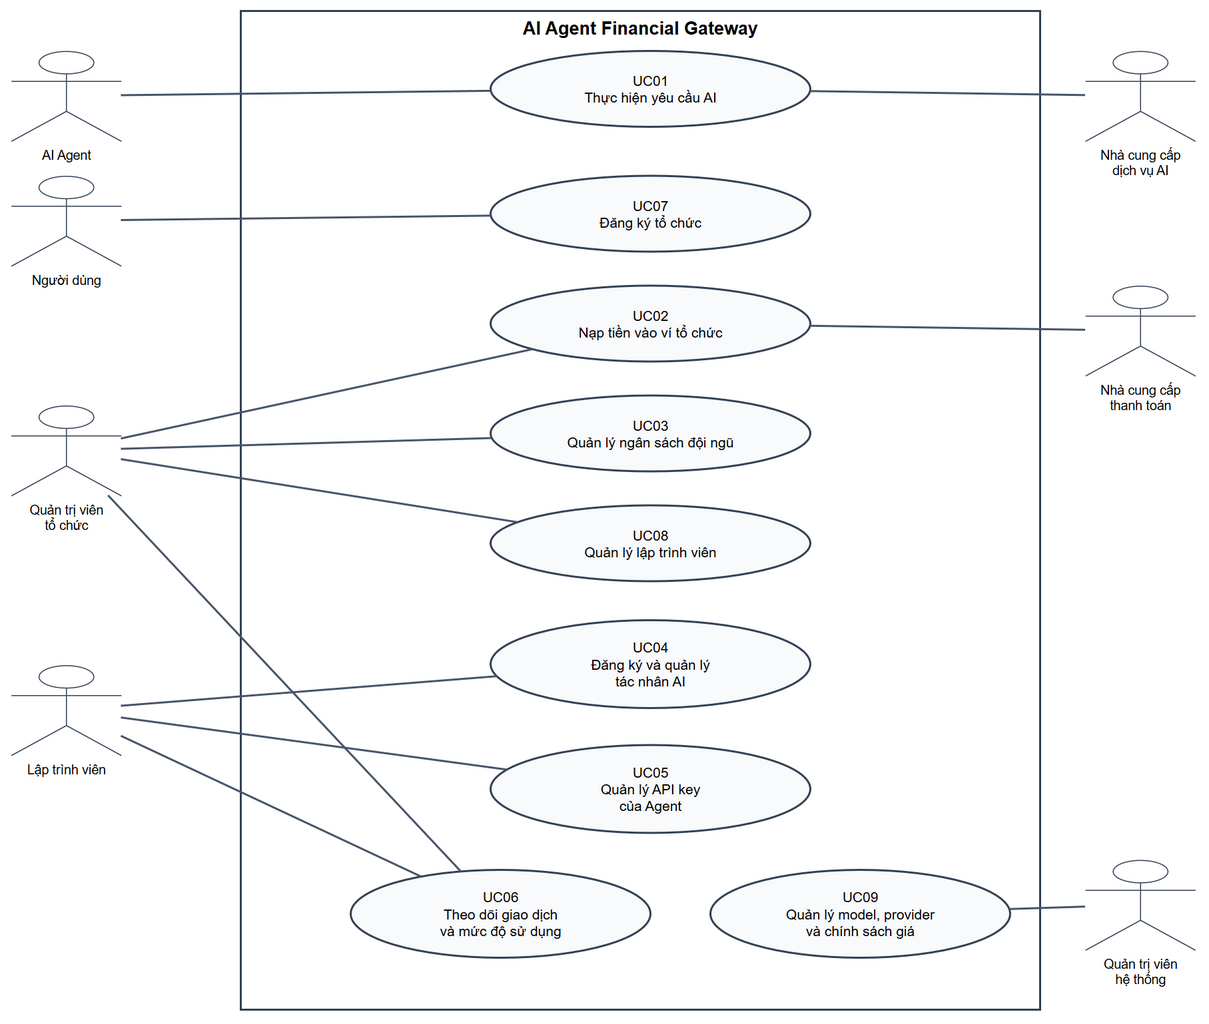
\includegraphics[width=1\textwidth]{images/2.3.1 Use case tổng quát.png}
    \caption[Biểu đồ trường hợp sử dụng tổng quát]{Biểu đồ trường hợp sử dụng tổng quát. Nguồn: Tác giả xây dựng}\label{fig:usecase}
\end{figure}
\section{Đặc tả trường hợp sử dụng}

Sau biểu đồ tổng quát, mỗi trường hợp sử dụng chính được trình bày bằng một biểu đồ chi tiết và một bảng đặc tả tương ứng. Biểu đồ chi tiết làm rõ Actor, phạm vi tương tác và các quan hệ include/extend nếu cần; bảng đặc tả mô tả thông tin chung, luồng chính, luồng thay thế, luồng ngoại lệ và hậu điều kiện. Cách trình bày này giúp liên kết trực tiếp giữa sơ đồ và kịch bản nghiệp vụ của từng Use Case.

\subsection*{UC01 - Thực hiện yêu cầu AI qua Gateway}

\begin{figure}[H]
    \centering
    
\includegraphics[width=0.92\textwidth]{report_support_documentation/use_cases/UC01/diagram.png}
    \caption[Biểu đồ trường hợp sử dụng UC01]{Biểu đồ trường hợp sử dụng UC01 -- Thực hiện yêu cầu AI qua Gateway. Nguồn: Tác giả xây dựng}
\end{figure}

\begin{longtable}{|L{4.2cm}|L{9.5cm}|}
\caption[Đặc tả UC01]{Đặc tả trường hợp sử dụng: UC01 -- Thực hiện yêu cầu AI qua Gateway} \\\hline
\textbf{Tên} & UC01: Thực hiện yêu cầu AI qua Gateway \\\hline
\textbf{Mô tả} & AI Agent muốn gửi yêu cầu qua Gateway để nhận kết quả AI theo luồng streaming trong phạm vi ngân sách được cấp.\\\hline
\textbf{Tác nhân} & Tác nhân chính: AI Agent.\newline Tác nhân hỗ trợ: Nhà cung cấp dịch vụ AI.\\\hline
\textbf{Mức ưu tiên} & Bắt buộc.\\\hline
\textbf{Sự kiện kích hoạt} & AI Agent gửi yêu cầu AI tới Gateway.\\\hline
\textbf{Điều kiện tiên quyết} & AI Agent đã được cấp API key của Gateway; chính sách ngân sách, danh mục mô hình, nhà cung cấp và biểu giá đã được thiết lập.\\\hline
\textbf{Luồng chính} &
1. AI Agent gửi API key, khóa lũy đẳng, nội dung tác vụ và các tùy chọn thực thi.\newline
2. Gateway xác thực yêu cầu và kiểm tra quyền thực thi.\newline
3. Gateway kiểm tra khóa lũy đẳng và ghi nhận yêu cầu mới.\newline
4. Gateway chọn phương án thực thi, kiểm tra chính sách và ngân sách liên quan.\newline
5. Gateway tạm giữ ngân sách cần thiết cho yêu cầu.\newline
6. Gateway dùng provider credential nội bộ để gọi nhà cung cấp dịch vụ AI và truyền từng phần kết quả cho AI Agent.\newline
7. Gateway xác định mức sử dụng thực tế sau khi luồng kết quả kết thúc.\newline
8. Gateway quyết toán chi phí, giải phóng phần còn dư và hoàn tất bản ghi lũy đẳng.\\\hline
\textbf{Luồng thay thế} &
\textbf{3a - Yêu cầu đã được xử lý:} 1. Gateway trả kết quả đã lưu và không gọi lại nhà cung cấp. 2. Use Case kết thúc thành công.\newline
\textbf{4a - Chọn phương án thay thế:} 1. Gateway chọn mô hình hoặc nhà cung cấp thay thế theo chính sách. 2. Use Case tiếp tục tại bước 5.\\\hline
\textbf{Luồng ngoại lệ} &
\textbf{2b - Yêu cầu hoặc quyền truy cập không hợp lệ:} 1. Gateway từ chối yêu cầu; không phát sinh tạm giữ ngân sách. 2. Use Case kết thúc không thành công.\newline
\textbf{4b - Không đủ ngân sách và không có phương án thay thế:} 1. Gateway xác định ngân sách hiện tại không đủ cho yêu cầu và không có mô hình hoặc nhà cung cấp thay thế phù hợp. 2. Gateway từ chối yêu cầu; không gọi nhà cung cấp dịch vụ AI và không phát sinh chi phí. 3. Use Case kết thúc không thành công.\newline
\textbf{6b - Luồng xử lý không hoàn tất:} 1. Gateway ghi nhận trạng thái lỗi, quyết toán phần chi phí đã phát sinh nếu có và chuyển giao dịch sang trạng thái có thể phục hồi hoặc đối soát. 2. Use Case kết thúc không thành công.\\\hline
\textbf{Hậu điều kiện thành công} & Kết quả đã được truyền cho AI Agent; chi phí thực tế đã được quyết toán; phần tạm giữ dư đã được giải phóng; nhật ký thực thi và bản ghi lũy đẳng đã hoàn tất.\\\hline
\textbf{Hậu điều kiện thất bại} & Không thực thi hoặc tính phí trùng; khoản tạm giữ được giải phóng hoặc chuyển sang trạng thái chờ xử lý; lỗi được lưu để thử lại hoặc đối soát.\\\hline
\textbf{Liên kết yêu cầu} & FR03, FR04, FR05, FR06, FR07, FR08, FR09, FR10; NFR01, NFR02, NFR03, NFR04, NFR05.\\\hline
\end{longtable}


\subsection*{UC02 - Nạp tiền vào ví tổ chức}

\begin{figure}[H]
    \centering
    
\includegraphics[width=0.92\textwidth]{report_support_documentation/use_cases/UC02/diagram.png}
    \caption[Biểu đồ trường hợp sử dụng UC02]{Biểu đồ trường hợp sử dụng UC02 -- Nạp tiền vào ví tổ chức. Nguồn: Tác giả xây dựng}
\end{figure}

\begin{longtable}{|L{4.2cm}|L{9.5cm}|}
\caption[Đặc tả UC02]{Đặc tả trường hợp sử dụng: UC02 -- Nạp tiền vào ví tổ chức} \\\hline
\textbf{Tên} & UC02: Nạp tiền vào ví tổ chức \\\hline
\textbf{Mô tả} & Quản trị viên tổ chức muốn nạp tiền vào ví tổ chức để tạo ngân sách sử dụng dịch vụ AI.\\\hline
\textbf{Tác nhân} & Tác nhân chính: Quản trị viên tổ chức.\newline Tác nhân hỗ trợ: Nhà cung cấp dịch vụ thanh toán.\\\hline
\textbf{Mức ưu tiên} & Bắt buộc.\\\hline
\textbf{Sự kiện kích hoạt} & Quản trị viên tổ chức yêu cầu nạp tiền.\\\hline
\textbf{Điều kiện tiên quyết} & Quản trị viên tổ chức đã đăng nhập; tổ chức và ví tổ chức đang hoạt động.\\\hline
\textbf{Luồng chính} &
1. Quản trị viên tổ chức nhập số tiền cần nạp và chọn phương thức thanh toán.\newline
2. Gateway kiểm tra số tiền nạp theo chính sách.\newline
3. Gateway tạo yêu cầu thanh toán và chuyển người dùng tới nhà cung cấp thanh toán.\newline
4. Quản trị viên hoàn tất thanh toán tại nhà cung cấp.\newline
5. Nhà cung cấp thanh toán gửi kết quả thanh toán về Gateway.\newline
6. Gateway xác thực kết quả thanh toán và kiểm tra giao dịch chưa được xử lý trước đó.\newline
7. Gateway cộng tiền vào ví tổ chức và ghi nhận bút toán.\newline
8. Gateway thông báo kết quả nạp tiền cho quản trị viên.\\\hline
\textbf{Luồng thay thế} &
\textbf{5a - Đối soát giao dịch nạp tiền:} 1. Nếu chưa nhận được callback thanh toán, Gateway giữ giao dịch ở trạng thái chờ. 2. Tiến trình đối soát tự động kiểm tra trạng thái thanh toán. 3. Nếu thanh toán thành công, Use Case tiếp tục tại bước 6.\\\hline
\textbf{Luồng ngoại lệ} &
\textbf{2b - Số tiền nạp không hợp lệ:} 1. Gateway từ chối yêu cầu và thông báo nguyên nhân. 2. Use Case kết thúc không thành công.\newline
\textbf{6b - Kết quả thanh toán không hợp lệ:} 1. Gateway từ chối cập nhật ví và ghi nhận giao dịch cần kiểm tra. 2. Use Case kết thúc không thành công.\newline
\textbf{7b - Cập nhật ví thất bại:} 1. Gateway không thay đổi số dư ví và giữ giao dịch ở trạng thái chờ xử lý. 2. Use Case kết thúc không thành công.\\\hline
\textbf{Hậu điều kiện thành công} & Ví tổ chức được cộng số tiền nạp hợp lệ; giao dịch nạp tiền và bút toán liên quan được ghi nhận.\\\hline
\textbf{Hậu điều kiện thất bại} & Số dư ví không thay đổi nếu thanh toán không hợp lệ; giao dịch lỗi được ghi nhận để đối soát.\\\hline
\textbf{Liên kết yêu cầu} & FR01, FR09; NFR01, NFR02, NFR03, NFR04.\\\hline
\end{longtable}


\subsection*{UC03 - Quản lý ngân sách tổ chức/team/developer}

\begin{figure}[H]
    \centering
    
\includegraphics[width=0.92\textwidth]{report_support_documentation/use_cases/UC03/diagram.png}
    \caption[Biểu đồ trường hợp sử dụng UC03]{Biểu đồ trường hợp sử dụng UC03 -- Quản lý ngân sách tổ chức/team/developer. Nguồn: Tác giả xây dựng}
\end{figure}

\begin{longtable}{|L{4.2cm}|L{9.5cm}|}
\caption[Đặc tả UC03]{Đặc tả trường hợp sử dụng: UC03 -- Quản lý ngân sách tổ chức/team/developer} \\\hline
\textbf{Tên} & UC03: Quản lý ngân sách tổ chức/team/developer \\\hline
\textbf{Mô tả} & Quản trị viên tổ chức muốn quản lý ngân sách đội ngũ để phân bổ hoặc thu hồi ngân sách sử dụng dịch vụ AI.\\\hline
\textbf{Tác nhân} & Tác nhân chính: Quản trị viên tổ chức.\newline Tác nhân hỗ trợ: Không có.\\\hline
\textbf{Mức ưu tiên} & Bắt buộc.\\\hline
\textbf{Sự kiện kích hoạt} & Quản trị viên tổ chức mở chức năng quản lý ngân sách đội ngũ.\\\hline
\textbf{Điều kiện tiên quyết} & Tổ chức đang hoạt động; lập trình viên mục tiêu thuộc tổ chức.\\\hline
\textbf{Luồng chính} &
1. Quản trị viên tổ chức mở chức năng quản lý ngân sách đội ngũ.\newline
2. Gateway hiển thị ngân sách khả dụng của tổ chức, danh sách lập trình viên, hạn mức hiện tại và lịch sử điều chuyển liên quan.\newline
3. Quản trị viên chọn thao tác phân bổ ngân sách cho một lập trình viên.\newline
4. Quản trị viên nhập số tiền cần phân bổ.\newline
5. Gateway kiểm tra số tiền phân bổ không vượt ngân sách khả dụng của tổ chức.\newline
6. Gateway điều chuyển ngân sách từ ví tổ chức sang hạn mức của lập trình viên.\newline
7. Gateway ghi nhận lịch sử điều chuyển và thông báo kết quả cho quản trị viên.\\\hline
\textbf{Luồng thay thế} &
\textbf{2a - Xem ngân sách tổ chức hoặc lập trình viên:} 1. Nếu chỉ cần tra cứu, quản trị viên xem ngân sách khả dụng của tổ chức hoặc hạn mức của từng lập trình viên. 2. Use Case kết thúc thành công.\newline
\textbf{2b - Xem lịch sử điều chuyển ngân sách:} 1. Nếu cần kiểm tra biến động ngân sách, quản trị viên chọn lịch sử điều chuyển. 2. Gateway hiển thị các lần phân bổ, thu hồi và trạng thái xử lý liên quan. 3. Use Case kết thúc thành công.\newline
\textbf{3a - Thu hồi ngân sách:} 1. Nếu cần thu hồi ngân sách, quản trị viên chọn thao tác thu hồi ngân sách của một lập trình viên. 2. Gateway hiển thị hạn mức hiện tại và phần ngân sách có thể thu hồi của lập trình viên. 3. Quản trị viên nhập số tiền cần thu hồi. 4. Gateway kiểm tra phần ngân sách có thể thu hồi. 5. Gateway điều chuyển ngân sách khả dụng về ví tổ chức và ghi nhận lịch sử điều chuyển. 6. Gateway thông báo kết quả cho quản trị viên. 7. Use Case kết thúc thành công.\newline
\textbf{5a - Ngân sách tổ chức không đủ:} 1. Gateway thông báo ngân sách khả dụng của tổ chức không đủ cho số tiền phân bổ. 2. Quản trị viên điều chỉnh số tiền phân bổ. 3. Use Case tiếp tục tại bước 5.\\\hline
\textbf{Luồng ngoại lệ} &
\textbf{3b - Lập trình viên không thuộc tổ chức:} 1. Gateway từ chối thao tác và giữ nguyên trạng thái ngân sách. 2. Use Case kết thúc không thành công.\newline
\textbf{3c - Số tiền thu hồi vượt phần khả dụng:} 1. Gateway từ chối phần thu hồi vượt quá ngân sách chưa cam kết. 2. Use Case kết thúc không thành công.\\\hline
\textbf{Hậu điều kiện thành công} & Hạn mức của lập trình viên và ví tổ chức được cập nhật nhất quán; lịch sử điều chuyển được ghi nhận.\\\hline
\textbf{Hậu điều kiện thất bại} & Không thay đổi số dư hoặc hạn mức khi yêu cầu không hợp lệ; lỗi được ghi nhận.\\\hline
\textbf{Liên kết yêu cầu} & FR01, FR05, FR09, FR10; NFR01, NFR02, NFR03.\\\hline
\end{longtable}


\subsection*{UC04 - Đăng ký và quản lý AI Agent}

\begin{figure}[H]
    \centering
    
\includegraphics[width=0.92\textwidth]{report_support_documentation/use_cases/UC04/diagram.png}
    \caption[Biểu đồ trường hợp sử dụng UC04]{Biểu đồ trường hợp sử dụng UC04 -- Đăng ký và quản lý AI Agent. Nguồn: Tác giả xây dựng}
\end{figure}

\begin{longtable}{|L{4.2cm}|L{9.5cm}|}
\caption[Đặc tả UC04]{Đặc tả trường hợp sử dụng: UC04 -- Đăng ký và quản lý AI Agent} \\\hline
\textbf{Tên} & UC04: Đăng ký và quản lý AI Agent \\\hline
\textbf{Mô tả} & Lập trình viên muốn đăng ký và quản lý tác nhân AI để hệ thống có thể kiểm soát trạng thái, hạn mức và chi phí phát sinh từ các yêu cầu AI.\\\hline
\textbf{Tác nhân} & Tác nhân chính: Lập trình viên.\newline Tác nhân hỗ trợ: Không có.\\\hline
\textbf{Mức ưu tiên} & Bắt buộc.\\\hline
\textbf{Sự kiện kích hoạt} & Lập trình viên mở chức năng đăng ký và quản lý tác nhân AI.\\\hline
\textbf{Điều kiện tiên quyết} & Lập trình viên đã đăng nhập và thuộc một tổ chức đang hoạt động.\\\hline
\textbf{Luồng chính} &
1. Lập trình viên mở chức năng đăng ký và quản lý tác nhân AI.\newline
2. Lập trình viên yêu cầu đăng ký tác nhân AI mới.\newline
3. Lập trình viên nhập tên, mô tả và phạm vi sử dụng dự kiến của tác nhân.\newline
4. Gateway kiểm tra thông tin đăng ký và gắn tác nhân với tổ chức của lập trình viên.\newline
5. Gateway tạo bản ghi tác nhân AI ở trạng thái hoạt động ban đầu.\newline
6. Gateway thông báo đăng ký thành công và cho phép lập trình viên tiếp tục thiết lập hạn mức hoặc API key.\\\hline
\textbf{Luồng thay thế} &
\textbf{2a - Xem thông tin tác nhân AI:} 1. Nếu chỉ cần tra cứu, lập trình viên xem thông tin đăng ký, hạn mức, phần đã sử dụng và trạng thái hiện tại của tác nhân AI. 2. Use Case kết thúc thành công.\newline
\textbf{3a - Thiết lập hạn mức tác nhân AI:} 1. Nếu cần kiểm soát chi phí, lập trình viên chọn một tác nhân AI đã đăng ký. 2. Gateway hiển thị hạn mức khả dụng của lập trình viên và chính sách hiện tại của tác nhân. 3. Lập trình viên nhập hạn mức và chu kỳ áp dụng. 4. Gateway kiểm tra hạn mức mới trong phạm vi ngân sách của lập trình viên. 5. Gateway lưu chính sách hạn mức mới và thông báo kết quả cho lập trình viên. 6. Use Case kết thúc thành công.\newline
\textbf{3b - Cập nhật chu kỳ ngân sách:} 1. Nếu cần thay đổi chu kỳ áp dụng, lập trình viên chọn thao tác cập nhật chu kỳ ngân sách. 2. Lập trình viên nhập chu kỳ mới. 3. Gateway kiểm tra chu kỳ hợp lệ và lưu chính sách mới. 4. Use Case kết thúc thành công.\newline
\textbf{3c - Tạm dừng tác nhân AI:} 1. Nếu cần dừng phát sinh chi phí mới, lập trình viên chọn tác nhân AI sau khi xem trạng thái hạn mức hiện tại. 2. Lập trình viên chọn thao tác tạm dừng tác nhân AI. 3. Gateway cập nhật trạng thái tác nhân và chặn các yêu cầu AI mới từ tác nhân này. 4. Use Case kết thúc thành công.\newline
\textbf{5a - Hạn mức mới thấp hơn mức đã sử dụng:} 1. Gateway ghi nhận chính sách mới nhưng chặn các yêu cầu mới vượt ngưỡng trong chu kỳ hiện tại. 2. Use Case kết thúc thành công.\\\hline
\textbf{Luồng ngoại lệ} &
\textbf{5b - Hạn mức vượt phạm vi được cấp:} 1. Gateway từ chối yêu cầu và giữ nguyên chính sách hiện tại. 2. Use Case kết thúc không thành công.\newline
\textbf{2b - Tác nhân không thuộc quyền quản lý:} 1. Gateway từ chối truy cập. 2. Use Case kết thúc không thành công.\newline
\textbf{4b - Thông tin tác nhân không hợp lệ:} 1. Gateway từ chối đăng ký tác nhân và thông báo trường dữ liệu cần điều chỉnh. 2. Use Case kết thúc không thành công.\\\hline
\textbf{Hậu điều kiện thành công} & Tác nhân AI được đăng ký hoặc cấu hình quản lý được cập nhật; trạng thái và chính sách hạn mức sẵn sàng cho UC01 kiểm soát yêu cầu.\\\hline
\textbf{Hậu điều kiện thất bại} & Chính sách hiện tại không thay đổi nếu yêu cầu không hợp lệ.\\\hline
\textbf{Liên kết yêu cầu} & FR02, FR05, FR09, FR10; NFR02, NFR03.\\\hline
\end{longtable}


\subsection*{UC05 - Quản lý API key của Agent}

\begin{figure}[H]
    \centering
    
\includegraphics[width=0.92\textwidth]{report_support_documentation/use_cases/UC05/diagram.png}
    \caption[Biểu đồ trường hợp sử dụng UC05]{Biểu đồ trường hợp sử dụng UC05 -- Quản lý API key của Agent. Nguồn: Tác giả xây dựng}
\end{figure}

\begin{longtable}{|L{4.2cm}|L{9.5cm}|}
\caption[Đặc tả UC05]{Đặc tả trường hợp sử dụng: UC05 -- Quản lý API key của Agent} \\\hline
\textbf{Tên} & UC05: Quản lý API key của Agent \\\hline
\textbf{Mô tả} & Lập trình viên muốn quản lý API key của Agent để kiểm soát quyền gọi Gateway của AI Agent.\\\hline
\textbf{Tác nhân} & Tác nhân chính: Lập trình viên.\newline Tác nhân hỗ trợ: Không có.\\\hline
\textbf{Mức ưu tiên} & Bắt buộc.\\\hline
\textbf{Sự kiện kích hoạt} & Lập trình viên yêu cầu quản lý API key của một AI Agent.\\\hline
\textbf{Điều kiện tiên quyết} & Lập trình viên đã đăng nhập; AI Agent thuộc quyền quản lý của lập trình viên.\\\hline
\textbf{Luồng chính} &
1. Lập trình viên chọn AI Agent cần quản lý API key.\newline
2. Gateway hiển thị danh sách API key hiện có của Agent.\newline
3. Lập trình viên yêu cầu tạo API key mới và nhập thông tin mô tả.\newline
4. Gateway tạo API key mới cho Agent.\newline
5. Gateway hiển thị giá trị API key một lần cho lập trình viên.\newline
6. Lập trình viên xác nhận đã lưu API key.\newline
7. Gateway kích hoạt API key và ghi nhận sự kiện bảo mật.\\\hline
\textbf{Luồng thay thế} &
\textbf{2a - Xem danh sách API key:} 1. Nếu chỉ cần tra cứu, lập trình viên xem danh sách API key và trạng thái của từng khóa. 2. Use Case kết thúc thành công.\newline
\textbf{3a - Thu hồi API key:} 1. Nếu cần thu hồi quyền truy cập, lập trình viên chọn một API key đang hoạt động từ danh sách API key. 2. Gateway thu hồi API key và ngăn khóa này xác thực các yêu cầu AI mới. 3. Use Case kết thúc thành công.\\\hline
\textbf{Luồng ngoại lệ} &
\textbf{1b - Agent không thuộc quyền quản lý:} 1. Gateway từ chối truy cập. 2. Use Case kết thúc không thành công.\newline
\textbf{4b - Không thể tạo API key:} 1. Gateway thông báo lỗi và không kích hoạt API key mới. 2. Use Case kết thúc không thành công.\\\hline
\textbf{Hậu điều kiện thành công} & API key của Agent được tạo hoặc thu hồi theo yêu cầu; trạng thái khóa được cập nhật trên Gateway.\\\hline
\textbf{Hậu điều kiện thất bại} & Không tạo hoặc thay đổi API key nếu yêu cầu không hợp lệ; sự kiện lỗi được ghi nhận.\\\hline
\textbf{Liên kết yêu cầu} & FR02, FR03, FR09, FR10; NFR02, NFR03.\\\hline
\end{longtable}


\subsection*{UC06 - Theo dõi giao dịch, usage, cost và trace}

\begin{figure}[H]
    \centering
    
\includegraphics[width=0.92\textwidth]{report_support_documentation/use_cases/UC06/diagram.png}
    \caption[Biểu đồ trường hợp sử dụng UC06]{Biểu đồ trường hợp sử dụng UC06 -- Theo dõi giao dịch, usage, cost và trace. Nguồn: Tác giả xây dựng}
\end{figure}

\begin{longtable}{|L{4.2cm}|L{9.5cm}|}
\caption[Đặc tả UC06]{Đặc tả trường hợp sử dụng: UC06 -- Theo dõi giao dịch, usage, cost và trace} \\\hline
\textbf{Tên} & UC06: Theo dõi giao dịch, usage, cost và trace \\\hline
\textbf{Mô tả} & Người dùng có quyền muốn theo dõi giao dịch và mức độ sử dụng để kiểm tra chi phí, usage và trace trong phạm vi được phân quyền.\\\hline
\textbf{Tác nhân} & Tác nhân chính: Quản trị viên tổ chức, Lập trình viên.\newline Tác nhân hỗ trợ: Không có.\\\hline
\textbf{Mức ưu tiên} & Bắt buộc.\\\hline
\textbf{Sự kiện kích hoạt} & Người dùng mở chức năng báo cáo sử dụng.\\\hline
\textbf{Điều kiện tiên quyết} & Người dùng đã đăng nhập và có quyền xem dữ liệu báo cáo.\\\hline
\textbf{Luồng chính} &
1. Người dùng mở chức năng theo dõi giao dịch và mức độ sử dụng.\newline
2. Gateway xác định vai trò và phạm vi dữ liệu được phép xem.\newline
3. Người dùng chọn tra cứu lịch sử giao dịch và nhập điều kiện lọc nếu cần.\newline
4. Gateway truy xuất giao dịch, bút toán và nhật ký thực thi phù hợp.\newline
5. Gateway hiển thị danh sách giao dịch và các chỉ số liên quan.\\\hline
\textbf{Luồng thay thế} &
\textbf{2a - Xem tổng quan mức sử dụng:} 1. Nếu chỉ cần tổng quan, người dùng chọn xem mức sử dụng theo phạm vi được phân quyền. 2. Gateway tổng hợp chi phí, usage và trạng thái giao dịch. 3. Gateway hiển thị chỉ số tổng quan. 4. Use Case kết thúc thành công.\newline
\textbf{3a - Lọc dữ liệu theo thời gian:} 1. Nếu cần thu hẹp phạm vi tra cứu, người dùng chọn khoảng thời gian hoặc điều kiện lọc. 2. Use Case tiếp tục tại bước 4.\newline
\textbf{5a - Không có dữ liệu phù hợp:} 1. Gateway hiển thị trạng thái không có dữ liệu. 2. Use Case kết thúc thành công.\newline
\textbf{5b - Xem chi tiết giao dịch:} 1. Người dùng chọn một giao dịch trong danh sách. 2. Gateway hiển thị chi tiết vòng đời yêu cầu, mức sử dụng, chi phí và nhật ký thực thi liên quan. 3. Use Case kết thúc thành công.\newline
\textbf{5c - Xuất báo cáo:} 1. Người dùng yêu cầu xuất dữ liệu báo cáo. 2. Gateway tạo tệp báo cáo theo phạm vi được phép. 3. Use Case kết thúc thành công.\\\hline
\textbf{Luồng ngoại lệ} &
\textbf{2b - Người dùng không có quyền:} 1. Gateway từ chối truy cập và không trả dữ liệu báo cáo. 2. Use Case kết thúc không thành công.\newline
\textbf{3b - Bộ lọc không hợp lệ:} 1. Gateway thông báo bộ lọc không hợp lệ và yêu cầu người dùng điều chỉnh điều kiện lọc. 2. Use Case kết thúc không thành công.\\\hline
\textbf{Hậu điều kiện thành công} & Người dùng nhận được dữ liệu giao dịch và mức sử dụng phù hợp với phạm vi quyền truy cập.\\\hline
\textbf{Hậu điều kiện thất bại} & Dữ liệu nhạy cảm không bị lộ khi người dùng không có quyền hoặc yêu cầu lọc không hợp lệ.\\\hline
\textbf{Liên kết yêu cầu} & FR01, FR02, FR09; NFR01, NFR02, NFR03.\\\hline
\end{longtable}


\subsection*{UC07 - Đăng ký tổ chức}

\begin{figure}[H]
    \centering
    
\includegraphics[width=0.92\textwidth]{report_support_documentation/use_cases/UC07/diagram.png}
    \caption[Biểu đồ trường hợp sử dụng UC07]{Biểu đồ trường hợp sử dụng UC07 -- Đăng ký tổ chức. Nguồn: Tác giả xây dựng}
\end{figure}

\begin{longtable}{|L{4.2cm}|L{9.5cm}|}
\caption[Đặc tả UC07]{Đặc tả trường hợp sử dụng: UC07 -- Đăng ký tổ chức} \\\hline
\textbf{Tên} & UC07: Đăng ký tổ chức \\\hline
\textbf{Mô tả} & Người dùng muốn đăng ký tổ chức mới để bắt đầu sử dụng hệ thống với vai trò quản trị viên tổ chức.\\\hline
\textbf{Tác nhân} & Tác nhân chính: Người dùng.\newline Tác nhân hỗ trợ: Không có.\\\hline
\textbf{Mức ưu tiên} & Bắt buộc.\\\hline
\textbf{Sự kiện kích hoạt} & Người dùng gửi yêu cầu tạo tổ chức.\\\hline
\textbf{Điều kiện tiên quyết} & Người dùng đã có danh tính hợp lệ; thông tin tổ chức chưa tồn tại trong hệ thống.\\\hline
\textbf{Luồng chính} &
1. Người dùng nhập thông tin tổ chức cần đăng ký.\newline
2. Gateway kiểm tra tính hợp lệ và tính duy nhất của thông tin tổ chức.\newline
3. Gateway khởi tạo tổ chức mới.\newline
4. Gateway gán người dùng hiện tại làm quản trị viên đầu tiên của tổ chức.\newline
5. Gateway tạo ví tổ chức với số dư ban đầu bằng không.\newline
6. Gateway thông báo đăng ký thành công và cho phép người dùng bắt đầu phiên làm việc.\\\hline
\textbf{Luồng thay thế} &
Không có.\\\hline
\textbf{Luồng ngoại lệ} &
\textbf{2b - Thông tin đăng ký không hợp lệ hoặc bị trùng:} 1. Gateway từ chối yêu cầu và thông báo trường dữ liệu cần điều chỉnh. 2. Use Case kết thúc không thành công.\newline
\textbf{3b - Khởi tạo tổ chức thất bại:} 1. Gateway hủy toàn bộ dữ liệu đã tạo trong yêu cầu đăng ký. 2. Use Case kết thúc không thành công.\\\hline
\textbf{Hậu điều kiện thành công} & Tổ chức mới được khởi tạo; người dùng hiện tại trở thành quản trị viên tổ chức; ví tổ chức được tạo.\\\hline
\textbf{Hậu điều kiện thất bại} & Không tạo dữ liệu tổ chức không hoàn chỉnh; lỗi được thông báo cho người đăng ký.\\\hline
\textbf{Liên kết yêu cầu} & FR01, FR09; NFR01, NFR02, NFR03.\\\hline
\end{longtable}


\subsection*{UC08 - Quản lý lập trình viên/thành viên tổ chức}

\begin{figure}[H]
    \centering
    
\includegraphics[width=0.92\textwidth]{report_support_documentation/use_cases/UC08/diagram.png}
    \caption[Biểu đồ trường hợp sử dụng UC08]{Biểu đồ trường hợp sử dụng UC08 -- Quản lý lập trình viên/thành viên tổ chức. Nguồn: Tác giả xây dựng}
\end{figure}

\begin{longtable}{|L{4.2cm}|L{9.5cm}|}
\caption[Đặc tả UC08]{Đặc tả trường hợp sử dụng: UC08 -- Quản lý lập trình viên/thành viên tổ chức} \\\hline
\textbf{Tên} & UC08: Quản lý lập trình viên/thành viên tổ chức \\\hline
\textbf{Mô tả} & Quản trị viên tổ chức muốn quản lý lập trình viên để kiểm soát thành viên, quyền truy cập và ngân sách trong tổ chức.\\\hline
\textbf{Tác nhân} & Tác nhân chính: Quản trị viên tổ chức.\newline Tác nhân hỗ trợ: Không có.\\\hline
\textbf{Mức ưu tiên} & Bắt buộc.\\\hline
\textbf{Sự kiện kích hoạt} & Quản trị viên tổ chức yêu cầu thay đổi danh sách lập trình viên.\\\hline
\textbf{Điều kiện tiên quyết} & Quản trị viên tổ chức đã đăng nhập; tổ chức đang hoạt động.\\\hline
\textbf{Luồng chính} &
1. Quản trị viên tổ chức mở chức năng quản lý lập trình viên.\newline
2. Gateway hiển thị danh sách lập trình viên và trạng thái hiện tại.\newline
3. Quản trị viên chọn thao tác tạo lập trình viên mới.\newline
4. Quản trị viên nhập thông tin lập trình viên.\newline
5. Gateway kiểm tra thông tin tài khoản và phạm vi tổ chức.\newline
6. Gateway tạo tài khoản lập trình viên, gắn với tổ chức và thiết lập hạn mức ban đầu.\newline
7. Gateway thông báo kết quả và cập nhật danh sách thành viên.\\\hline
\textbf{Luồng thay thế} &
\textbf{2a - Xem chi tiết lập trình viên:} 1. Nếu cần tra cứu, quản trị viên chọn một lập trình viên trong danh sách. 2. Gateway hiển thị thông tin tài khoản, hạn mức, Agent liên quan và trạng thái API key. 3. Use Case kết thúc thành công.\newline
\textbf{3a - Cập nhật thông tin lập trình viên:} 1. Nếu cần thay đổi thông tin, quản trị viên chọn lập trình viên cần cập nhật. 2. Quản trị viên nhập thông tin cần thay đổi. 3. Gateway kiểm tra dữ liệu và cập nhật thông tin lập trình viên. 4. Use Case kết thúc thành công.\newline
\textbf{3b - Vô hiệu hóa lập trình viên:} 1. Nếu cần ngừng quyền sử dụng, quản trị viên chọn lập trình viên cần vô hiệu hóa. 2. Gateway ngăn lập trình viên thực hiện thao tác mới. 3. Gateway thực hiện UC05.3 để thu hồi các API key liên quan. 4. Gateway thu hồi phần ngân sách khả dụng về ví tổ chức. 5. Use Case kết thúc thành công.\\\hline
\textbf{Luồng ngoại lệ} &
\textbf{5b - Email đã tồn tại hoặc dữ liệu không hợp lệ:} 1. Gateway từ chối yêu cầu và thông báo nguyên nhân. 2. Use Case kết thúc không thành công.\newline
\textbf{3c - Lập trình viên còn giao dịch chưa quyết toán:} 1. Khi vô hiệu hóa lập trình viên còn giao dịch chưa quyết toán, Gateway chặn yêu cầu mới và chuyển phần ngân sách liên quan sang chờ xử lý. 2. Use Case kết thúc không thành công một phần.\\\hline
\textbf{Hậu điều kiện thành công} & Tài khoản lập trình viên và quyền truy cập liên quan được cập nhật theo yêu cầu.\\\hline
\textbf{Hậu điều kiện thất bại} & Không thay đổi tài khoản hoặc ngân sách nếu yêu cầu không hợp lệ.\\\hline
\textbf{Liên kết yêu cầu} & FR01, FR02, FR05, FR09, FR10; NFR01, NFR02, NFR03.\\\hline
\end{longtable}


\subsection*{UC09 - Quản lý model, provider và chính sách giá}

\begin{figure}[H]
    \centering
    
\includegraphics[width=0.92\textwidth]{report_support_documentation/use_cases/UC09/diagram.png}
    \caption[Biểu đồ trường hợp sử dụng UC09]{Biểu đồ trường hợp sử dụng UC09 -- Quản lý model, provider và chính sách giá. Nguồn: Tác giả xây dựng}
\end{figure}

\begin{longtable}{|L{4.2cm}|L{9.5cm}|}
\caption[Đặc tả UC09]{Đặc tả trường hợp sử dụng: UC09 -- Quản lý model, provider và chính sách giá} \\\hline
\textbf{Tên} & UC09: Quản lý model, provider và chính sách giá \\\hline
\textbf{Mô tả} & Quản trị viên hệ thống muốn quản lý provider, model và chính sách giá để Gateway định tuyến, ước lượng chi phí và tính phí request AI.\\\hline
\textbf{Tác nhân} & Tác nhân chính: Quản trị viên hệ thống.\newline Tác nhân hỗ trợ: Không có.\\\hline
\textbf{Mức ưu tiên} & Bắt buộc.\\\hline
\textbf{Sự kiện kích hoạt} & Quản trị viên hệ thống yêu cầu cập nhật provider, model hoặc chính sách giá.\\\hline
\textbf{Điều kiện tiên quyết} & Quản trị viên hệ thống đã đăng nhập.\\\hline
\textbf{Luồng chính} &
1. Quản trị viên hệ thống mở chức năng quản lý model, provider và chính sách giá.\newline
2. Gateway hiển thị trạng thái provider, model, provider credential và chính sách giá hiện tại.\newline
3. Quản trị viên chọn thao tác cập nhật thông tin model hoặc provider.\newline
4. Quản trị viên nhập thông tin cần thay đổi.\newline
5. Gateway kiểm tra cấu hình mới theo quy tắc hợp lệ.\newline
6. Gateway lưu cấu hình model hoặc provider.\newline
7. Gateway thông báo cấu hình đã sẵn sàng cho các yêu cầu tiếp theo.\\\hline
\textbf{Luồng thay thế} &
\textbf{2a - Xem danh mục model/provider:} 1. Nếu chỉ cần tra cứu, quản trị viên hệ thống xem danh mục model, provider, trạng thái hỗ trợ và biểu giá hiện tại. 2. Use Case kết thúc thành công.\newline
\textbf{3a - Thêm model/provider:} 1. Nếu cần bổ sung cấu hình mới, quản trị viên hệ thống chọn thao tác thêm model hoặc provider. 2. Quản trị viên nhập thông tin cấu hình, trạng thái hỗ trợ và biểu giá ban đầu nếu có. 3. Gateway kiểm tra dữ liệu và lưu cấu hình mới. 4. Use Case kết thúc thành công.\newline
\textbf{3b - Vô hiệu hóa model:} 1. Nếu cần ngừng sử dụng một model, quản trị viên hệ thống chọn model từ danh mục model/provider. 2. Quản trị viên hệ thống chọn thao tác vô hiệu hóa model. 3. Gateway ngừng chọn model này cho yêu cầu mới. 4. Use Case kết thúc thành công.\newline
\textbf{3c - Cập nhật biểu giá:} 1. Nếu cần thay đổi biểu giá, quản trị viên hệ thống chọn model hoặc provider từ danh mục. 2. Quản trị viên hệ thống nhập giá mới và thời điểm hiệu lực. 3. Gateway lưu biểu giá mới, không làm thay đổi các giao dịch đã quyết toán. 4. Use Case kết thúc thành công.\newline
\textbf{3d - Thiết lập chính sách fallback:} 1. Nếu cần phương án dự phòng, quản trị viên hệ thống chọn model hoặc provider gốc từ danh mục. 2. Quản trị viên hệ thống cấu hình model hoặc provider thay thế. 3. Gateway lưu chính sách fallback để UC01 sử dụng khi model ban đầu không khả dụng hoặc không phù hợp với ngân sách. 4. Use Case kết thúc thành công.\newline
\textbf{3e - Model đang được sử dụng trong request đang xử lý:} 1. Nếu model đang được request sử dụng, Gateway áp dụng thay đổi cho yêu cầu mới và giữ nguyên cấu hình cũ cho request đang xử lý. 2. Use Case kết thúc thành công có điều kiện.\\\hline
\textbf{Luồng ngoại lệ} &
\textbf{5b - Cấu hình không hợp lệ:} 1. Gateway từ chối thay đổi và giữ nguyên cấu hình hiện tại. 2. Use Case kết thúc không thành công.\\\hline
\textbf{Hậu điều kiện thành công} & Cấu hình provider, model và chính sách giá được cập nhật; Gateway có thể sử dụng cấu hình mới cho các yêu cầu tiếp theo.\\\hline
\textbf{Hậu điều kiện thất bại} & Cấu hình hiện tại không thay đổi nếu dữ liệu mới không hợp lệ hoặc gây xung đột.\\\hline
\textbf{Liên kết yêu cầu} & FR04, FR05, FR07, FR09; NFR02, NFR03, NFR04.\\\hline
\end{longtable}

\section{Mô hình hóa luồng nghiệp vụ}

Các biểu đồ hoạt động mô tả thứ tự xử lý, điều kiện rẽ nhánh và trạng thái kết thúc của những luồng nghiệp vụ quan trọng trong hệ thống. Ba luồng được ưu tiên gồm: AI Agent gọi dịch vụ AI qua Gateway, đăng ký AI Agent và cấp API key, nạp tiền và phân bổ ngân sách.

\begin{figure}[htbp]
    \centering
    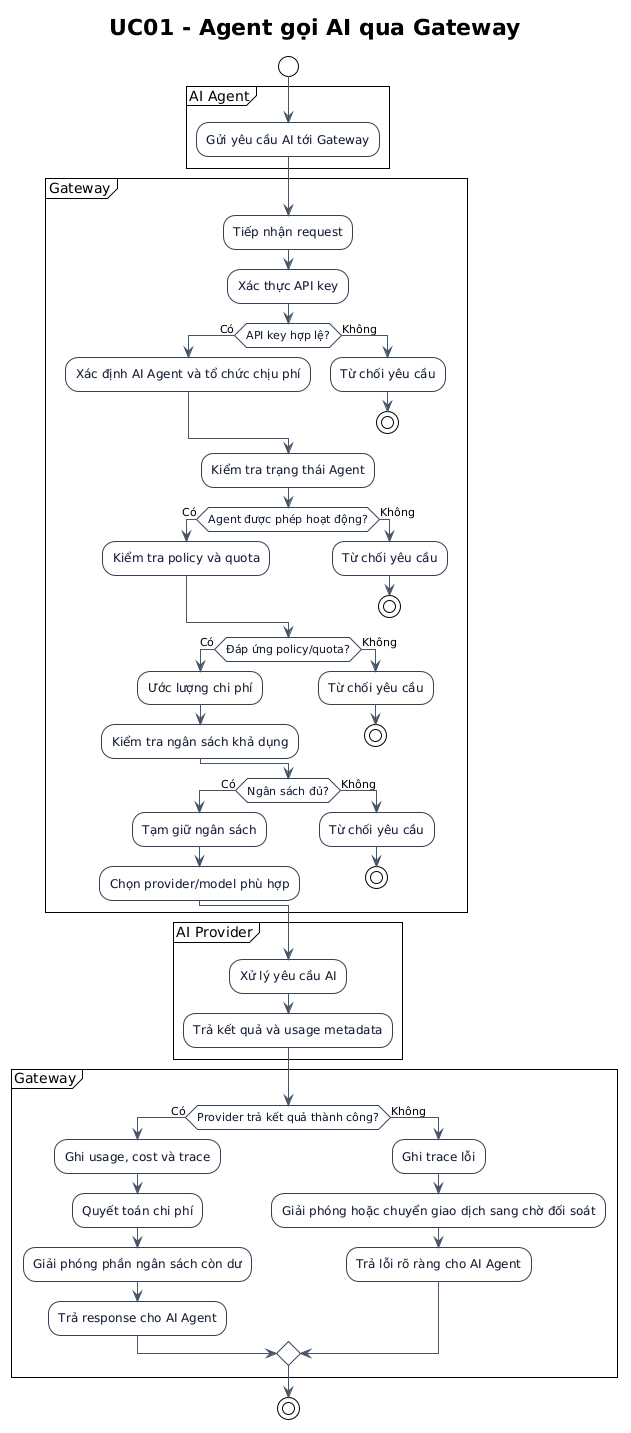
\includegraphics[height=0.86\textheight,keepaspectratio]{report_support_documentation/activity_diagrams/UC01/activity.png}
    \caption[Biểu đồ hoạt động UC01]{Biểu đồ hoạt động UC01 -- Luồng xử lý yêu cầu AI qua Gateway. Nguồn: Tác giả xây dựng}\label{fig:activity-uc01-ai-request}
\end{figure}

\cref{fig:activity-uc01-ai-request} cho thấy yêu cầu bị từ chối sớm nếu xác thực thất bại, khóa lũy đẳng xung đột hoặc ngân sách không đáp ứng điều kiện. Nếu yêu cầu đã hoàn tất trước đó, hệ thống trả kết quả đã lưu mà không tạo giao dịch mới.

Với yêu cầu mới, Gateway ước lượng chi phí, xác định giới hạn đầu ra và tạm giữ ngân sách trước khi gọi nhà cung cấp. Sau khi nhận kết quả, hệ thống tính chi phí thực tế, quyết toán phần đã sử dụng, giải phóng phần còn dư và lưu nhật ký thực thi. Luồng này mô tả thiết kế mục tiêu; nguyên mẫu hiện tại mới triển khai thu phí cố định trước khi chuyển tiếp yêu cầu.

\begin{figure}[htbp]
    \centering
    
\includegraphics[height=0.82\textheight,keepaspectratio]{report_support_documentation/activity_diagrams/UC04_agent_registration/activity.png}
    \caption[Biểu đồ hoạt động đăng ký AI Agent]{Biểu đồ hoạt động đăng ký AI Agent và cấp API key. Nguồn: Tác giả xây dựng}\label{fig:activity-agent-registration}
\end{figure}

\cref{fig:activity-agent-registration} làm rõ hệ thống không tạo, huấn luyện hoặc vận hành AI Agent. Gateway chỉ ghi nhận Agent bên ngoài vào hệ thống, gắn Agent với tổ chức, sinh API key do Asymptotic quản lý và trả khóa cho người dùng có quyền để cấu hình Agent ở bên ngoài.

\begin{figure}[htbp]
    \centering
    
\includegraphics[height=0.82\textheight,keepaspectratio]{report_support_documentation/activity_diagrams/finance_budget/activity.png}
    \caption[Biểu đồ hoạt động nạp tiền và phân bổ ngân sách]{Biểu đồ hoạt động nạp tiền và phân bổ ngân sách. Nguồn: Tác giả xây dựng}\label{fig:activity-finance-budget}
\end{figure}

\cref{fig:activity-finance-budget} mô tả luồng tài chính trước khi Agent phát sinh chi phí. Tổ chức cần nạp tiền vào ví, Gateway xác thực kết quả thanh toán và ghi nhận bút toán, sau đó quản trị viên tổ chức phân bổ ngân sách cho Agent hoặc nhóm sử dụng phù hợp.

\section*{Kết luận chương}

Chương này đã khảo sát hiện trạng, xác định yêu cầu chức năng và phi chức năng, mô tả các trường hợp sử dụng chính và mô hình hóa luồng nghiệp vụ trung tâm bằng biểu đồ hoạt động. Các kết quả này là cơ sở cho phân tích lớp hướng đối tượng trong Chương 3 và thiết kế chi tiết trong Chương 4. Phạm vi triển khai thực tế được đối chiếu riêng tại Chương 5.
